%% This file contains 6 slides
\begin{slide}
Redes Neurais Artificiais - O neur�nio artificial

\begin{center}
{\tiny \input{picts/neuronc.pic}}
\end{center}
RNA multi-camadas

\begin{center}
{\tiny \input{picts/multi.pic}}
\end{center}
\end{slide}

\begin{slide}
O Sistema TN310

\begin{itemize} 
 \item Processamento Distribu�do
 \item 16 n�s independentes
 \item Mem�ria Local (MIMD)
 \item HTRAM-s tamanho 4
 \begin{enumerate} 
  \item T9000
  \item ADSP 21020 (196Kbytes)
  \item 8Mbytes RAM
  \item 256Kbytes \eng{shared}
 \end{enumerate}
 \item Totalmente conectado atrav�s de chaves STC104
\end{itemize}
\end{slide}

\begin{slide}
O T9000

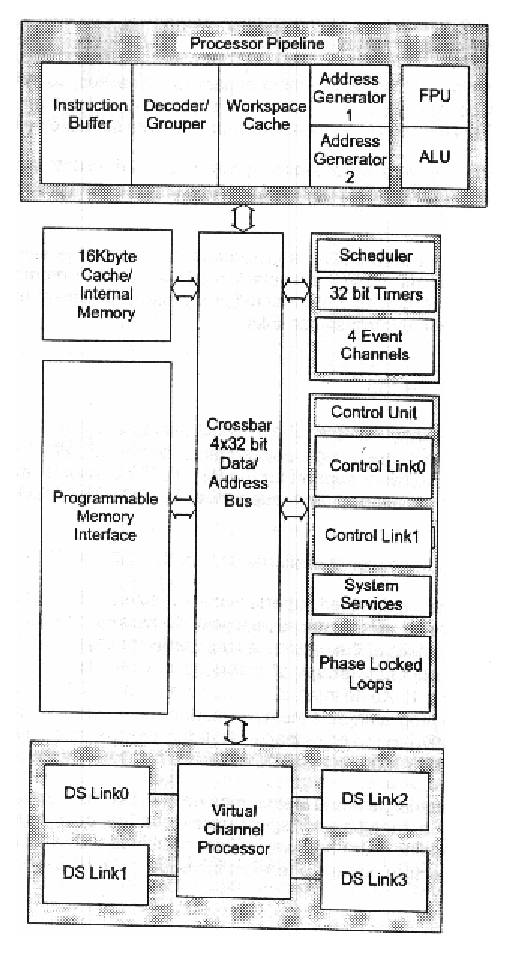
\includegraphics[type=eps, ext=.eps, bb= 0 0 228 441]{figs/T9000}
\end{slide}

\begin{slide}
O ADSP 21020

\end{slide}

\begin{slide}
A conex�o entre os n�s na TN310

{\tiny \input{picts/connect2.pic}}
\end{slide}

\begin{slide}
N�veis de programa��o

\begin{center}
{\tiny \input{picts/layer.pic}}
\end{center}

Comunica��o por canais
\begin{center}
{\tiny \input{picts/chan_op2.pic}}
\end{center}
\end{slide}


